\documentclass[journal]{IEEEtran}

% =========================================================================
% REQUIRED PACKAGES & CONFIGURATION
% =========================================================================
\usepackage{cite}
\usepackage{amsmath,amssymb,amsfonts}
\usepackage{algorithmic}
\usepackage{algorithm}
\usepackage{graphicx}
\usepackage{textcomp}
\usepackage{xcolor}
\usepackage{booktabs}
\usepackage{multirow}
\usepackage{microtype}
\usepackage{url}

\hyphenation{op-tical net-works semi-conduc-tor Agro-Vision}

\begin{document}

\title{AgroVision: An Explainable Deep Transfer Learning Architecture for Foliar Pathology Classification Across Multi-Crop Benchmarks}

\author{Thummala~Charan~Chowdary,
        K.~Dinesh~Karthik,
        and~A.~Hareeshwar~Goud%
\thanks{Manuscript submitted to Dr. Pujari Jeevana Jyothi for CSE 4006: Deep Learning Course Project, School of Computer Science and Engineering (SCOPE), VIT-AP University, Amaravati, Andhra Pradesh 522237, India.}%
\thanks{Authors are undergraduate scholars at VIT-AP University (e-mail: charan.24bca7633@vitapstudent.ac.in, dinesh.karthik@vitapstudent.ac.in, hareeshwar.goud@vitapstudent.ac.in).}}

\markboth{VIT-AP University, SCOPE, CSE 4006: Deep Learning, October 2026}%
{Chowdary \MakeLowercase{\textit{et al.}}: AgroVision: Explainable Deep Transfer Learning for Foliar Pathology}

\maketitle

% =========================================================================
% ABSTRACT & INDEX TERMS
% =========================================================================
\begin{abstract}
Phytopathogenic foliar diseases represent a persistent structural hazard to global agricultural yield, food supply stability, and commercial farming viability. While deep convolutional neural network (CNN) architectures have achieved unprecedented classification benchmarks on curated datasets, operational integration requires rigorous comparative evaluation, statistical significance verification, and transparent decision explainability. In this paper, we develop \textbf{AgroVision}, an explainable deep transfer learning framework for foliar pathology diagnosis across 38 semantic categories spanning 14 crop species in the PlantVillage benchmark. We conduct an exhaustive multi-backbone comparative study evaluating a custom 4-stage convolutional baseline against two transfer learning topologies: ResNet-50 and EfficientNet-B0. On an independent held-out test split of 8,146 samples, ResNet-50 demonstrated superior discriminative capability, achieving an overall top-1 accuracy of 97.88\% (Macro Precision: 0.9726, Macro Recall: 0.9692, Macro F1-score: 0.9706), significantly outperforming EfficientNet-B0 (96.34\% accuracy, Macro F1: 0.9515) and the Custom CNN baseline (94.61\% accuracy, Macro F1: 0.9284). Pairwise McNemar statistical hypothesis tests confirm that the observed performance divergences are statistically significant ($\chi^2 = 142.16$, $p = 8.99 \times 10^{-33}$ between Custom CNN and ResNet-50). To eliminate decision opacity, we integrate Gradient-weighted Class Activation Mapping (Grad-CAM), confirming that the network's spatial attention is anchored directly to pathological lesions rather than contextual background artifacts.
\end{abstract}

\begin{IEEEkeywords}
Plant disease detection, deep transfer learning, ResNet-50, EfficientNet-B0, Custom CNN, McNemar statistical test, Grad-CAM, explainable artificial intelligence (XAI), computer vision.
\end{IEEEkeywords}

% =========================================================================
% SECTION I: INTRODUCTION
% =========================================================================
\section{Introduction}
\IEEEPARstart{A}{gricultural} crop losses driven by phytopathogenic infestations impose severe macroeconomic burdens worldwide, causing an estimated 20\% to 40\% loss in global harvest yield across primary staples annually~\cite{hughes2015, mohanty2016, savary2019}. The rapid spread of fungal pathogens, bacterial spot agents, and viral strains threatens food security and destabilizes market pricing~\cite{barbedo2013}. Diagnostic appraisal has historically relied on physical scouting by extension workers or laboratory assays such as polymerase chain reaction (PCR) and enzyme-linked immunosorbent assay (ELISA)~\cite{martin2000, sankaran2010}. Although molecular assays offer high analytical precision, they require sophisticated laboratory equipment, cold-chain transport, expensive chemical reagents, and multi-day turnaround periods~\cite{sankaran2010}. Consequently, rapid automated visual screening directly from photographic leaf samples is essential.

Deep convolutional neural networks (CNNs) have set state-of-the-art benchmarks in computer vision by autonomously learning hierarchical representations directly from raw pixel arrays~\cite{krizhevsky2012, lecun2015}. Applied to agricultural imagery, deep learning models have achieved high classification accuracy on curated benchmarks~\cite{ferentinos2018, too2019, chen2020}. However, standard high-capacity networks operate with vast parameter counts and non-linear layer stacks that present two core challenges:

\begin{enumerate}
    \item \textbf{Architectural Efficiency and Inductive Bias:} High-capacity models such as standard ResNet-50~\cite{he2016} (23.5M parameters) rely on residual bottleneck shortcuts, whereas inverted residual topologies like EfficientNet-B0~\cite{tan2019} leverage compound scaling and depthwise separable convolutions (4.0M parameters). Quantifying the exact trade-off between parameter footprint, computational convergence, and classification accuracy across fine-grained botanical classes requires systematic empirical evaluation.
    \item \textbf{Decision Opacity (Black-Box Problem):} Standard deep learning architectures operate without visual explanations~\cite{selvaraju2017}. In agricultural diagnostics, where erroneous classifications can lead to incorrect chemical usage or crop failure, practitioners must verify whether predictions stem from actual pathological symptoms or background artifacts such as soil, shadows, or lighting variations~\cite{chouhan2020}.
\end{enumerate}

\subsection{Research Objectives and Scope}
To resolve these challenges, this study presents \textbf{AgroVision}, an empirical and explainable deep learning framework. We evaluate a lightweight Custom CNN against ResNet-50~\cite{he2016} and EfficientNet-B0~\cite{tan2019}. We structure our investigation around four central research questions:
\begin{itemize}
    \item \textbf{RQ1:} How do residual skip connections versus inverted residual bottlenecks affect feature representations and classification accuracy across 38 distinct crop-pathology categories?
    \item \textbf{RQ2:} Can parameter-efficient backbones (e.g., EfficientNet-B0) deliver classification performance competitive with heavily parameterized residual networks (e.g., ResNet-50) under equivalent training conditions?
    \item \textbf{RQ3:} Are observed empirical differences across model families statistically significant, or can they be attributed to random test sampling variance?
    \item \textbf{RQ4:} Can visual saliency maps generated via Grad-CAM~\cite{selvaraju2017} verify that models focus on authentic necrotic lesions?
\end{itemize}

\subsection{Contributions}
This paper makes four main contributions:
\begin{enumerate}
    \item We design and systematically evaluate a multi-backbone agricultural diagnostic pipeline benchmarked across 54,305 images spanning 38 classes in the PlantVillage repository.
    \item We perform a quantitative comparison of ResNet-50 (97.88\%), EfficientNet-B0 (96.34\%), and a baseline Custom CNN (94.61\%), analyzing convergence dynamics and trade-offs between parameter efficiency and accuracy.
    \item We conduct pairwise McNemar statistical hypothesis tests ($\alpha = 0.05$) to establish whether differences in classifier performance are statistically significant.
    \item We incorporate an explainable AI pipeline using Grad-CAM to validate feature attributions, confirming that gradient attention localizes over authentic pathological tissue.
\end{enumerate}

% =========================================================================
% SECTION II: RELATED WORK & SYSTEMATIC TAXONOMY
% =========================================================================
\section{Related Work}

\subsection{Handcrafted Feature Extraction and Classical ML}
Initial efforts in automated foliar pathology diagnosis relied on handcrafted feature extraction pipelines. Researchers utilized Gray-Level Co-occurrence Matrices (GLCM) to capture leaf texture statistics, color space transformations (converting RGB into HSV and CIE $L^*a^*b^*$) to isolate chlorosis and necrosis, and Scale-Invariant Feature Transform (SIFT) descriptors to detect lesion edges~\cite{camargo2009, revathi2012}. Extracted feature vectors were subsequently categorized using classical classifiers such as Support Vector Machines (SVM)~\cite{cortes1995}, $k$-Nearest Neighbors ($k$-NN), and Random Forests~\cite{breiman2001}. 

While these methods were computationally lightweight, they exhibited fragile generalization under variable lighting, leaf surface reflections, scale transformations, and background noise~\cite{barbedo2013}. Consequently, these pipelines could not reliably scale across diverse crop species or varying disease severities.

\subsection{Deep Convolutional Architectures in Agriculture}
The release of curated agricultural repositories, particularly the PlantVillage dataset~\cite{hughes2015}, spurred the adoption of deep convolutional neural networks. Mohanty \textit{et al.}~\cite{mohanty2016} benchmarked AlexNet~\cite{krizhevsky2012} and GoogLeNet~\cite{szegedy2015} across 54,306 images, achieving classification accuracies exceeding 99\% under controlled imaging conditions. Ferentinos~\cite{ferentinos2018} expanded this scope by evaluating VGG-16, VGG-19, and ResNet architectures across 58 distinct classes, demonstrating that deeper networks improved feature discrimination but required large parameter footprints ($>138\text{M}$ weights for VGG-16). 

Too \textit{et al.}~\cite{too2019} evaluated DenseNet-121, Inception-V4, ResNet-50, and VGG-16, observing that DenseNet-121 achieved an accuracy of 99.75\% due to feature reuse across densely connected layers. Similarly, Chen \textit{et al.}~\cite{chen2020} demonstrated transfer learning across complex field backgrounds. However, these investigations focused primarily on raw accuracy while giving limited attention to parameter trade-offs, formal hypothesis testing, or visual explainability.

\begin{table*}[t]
\caption{Systematic Comparative Review of Contemporary Agricultural Diagnostic Architectures}
\label{tab:lit_comparison}
\centering
\begin{tabular*}{\textwidth}{@{\extracolsep{\fill}}lcccccc}
\toprule
\textbf{Framework} & \textbf{Core Backbone} & \textbf{Parameters (M)} & \textbf{Classes} & \textbf{Reported Metric} & \textbf{Statistical Test} & \textbf{XAI Module} \\
\midrule
Mohanty \textit{et al.}~\cite{mohanty2016} & AlexNet / GoogLeNet & 60.0 / 7.0 & 38 & 99.35\% Acc. & None & Absent \\
Ferentinos~\cite{ferentinos2018} & VGG-16 / ResNet-50 & 138.0 / 25.6 & 58 & 99.53\% Acc. & None & Absent \\
Too \textit{et al.}~\cite{too2019} & DenseNet-121 & 8.0 & 38 & 99.75\% Acc. & None & Absent \\
Chen \textit{et al.}~\cite{chen2020} & MobileNetV1 & 4.2 & 10 & 96.20\% Acc. & None & CAM \\
Chouhan \textit{et al.}~\cite{chouhan2020} & Custom CNN & 5.6 & 4 & 95.80\% Acc. & None & Grad-CAM \\
\textbf{AgroVision (Ours)} & \textbf{ResNet-50 / EffNet-B0} & \textbf{23.5 / 4.0} & \textbf{38} & \textbf{97.88\% / 96.34\%} & \textbf{McNemar ($\mathbf{p < 0.001}$)} & \textbf{Grad-CAM} \\
\bottomrule
\end{tabular*}
\end{table*}

\subsection{Model Efficiency, Compression, and Lightweight Topologies}
To optimize deep learning models, researchers developed parameter-efficient convolutional blocks. Howard \textit{et al.}~\cite{howard2017} introduced MobileNetV1, factorizing standard convolutions into depthwise and pointwise operations. Sandler \textit{et al.}~\cite{sandler2018} introduced inverted residuals and linear bottlenecks in MobileNetV2. Tan and Le~\cite{tan2019} developed EfficientNet, proposing a compound scaling principle that simultaneously scales depth, width, and resolution using neural architecture search. Table~\ref{tab:lit_comparison} contrasts AgroVision against contemporary agricultural diagnostic frameworks.

\subsection{Explainable Artificial Intelligence (XAI)}
Deploying automated diagnostic systems in agricultural domains requires interpretable decision-making. Techniques such as Class Activation Mapping (CAM)~\cite{zhou2016} and Gradient-weighted Class Activation Mapping (Grad-CAM)~\cite{selvaraju2017} calculate gradient-weighted spatial saliency maps, revealing the input regions that most influence network predictions. Visual heatmaps allow users to verify that model classifications are driven by genuine disease lesions rather than background artifacts~\cite{chouhan2020, singh2020}.

% =========================================================================
% SECTION III: ARCHITECTURAL DESIGN & METHODOLOGY
% =========================================================================
\section{Architectural Design and Methodology}

The multi-level system architecture, encompassing the macro feature extraction pipeline, internal bottleneck building block dynamics, and explainability mechanisms, is illustrated in Fig.~\ref{fig:building_blocks} and Fig.~\ref{fig:system_pipeline}.

% FIGURE 1: EXPANDED COMFORTABLE DOUBLE COLUMN
\begin{figure*}[t]
\centering
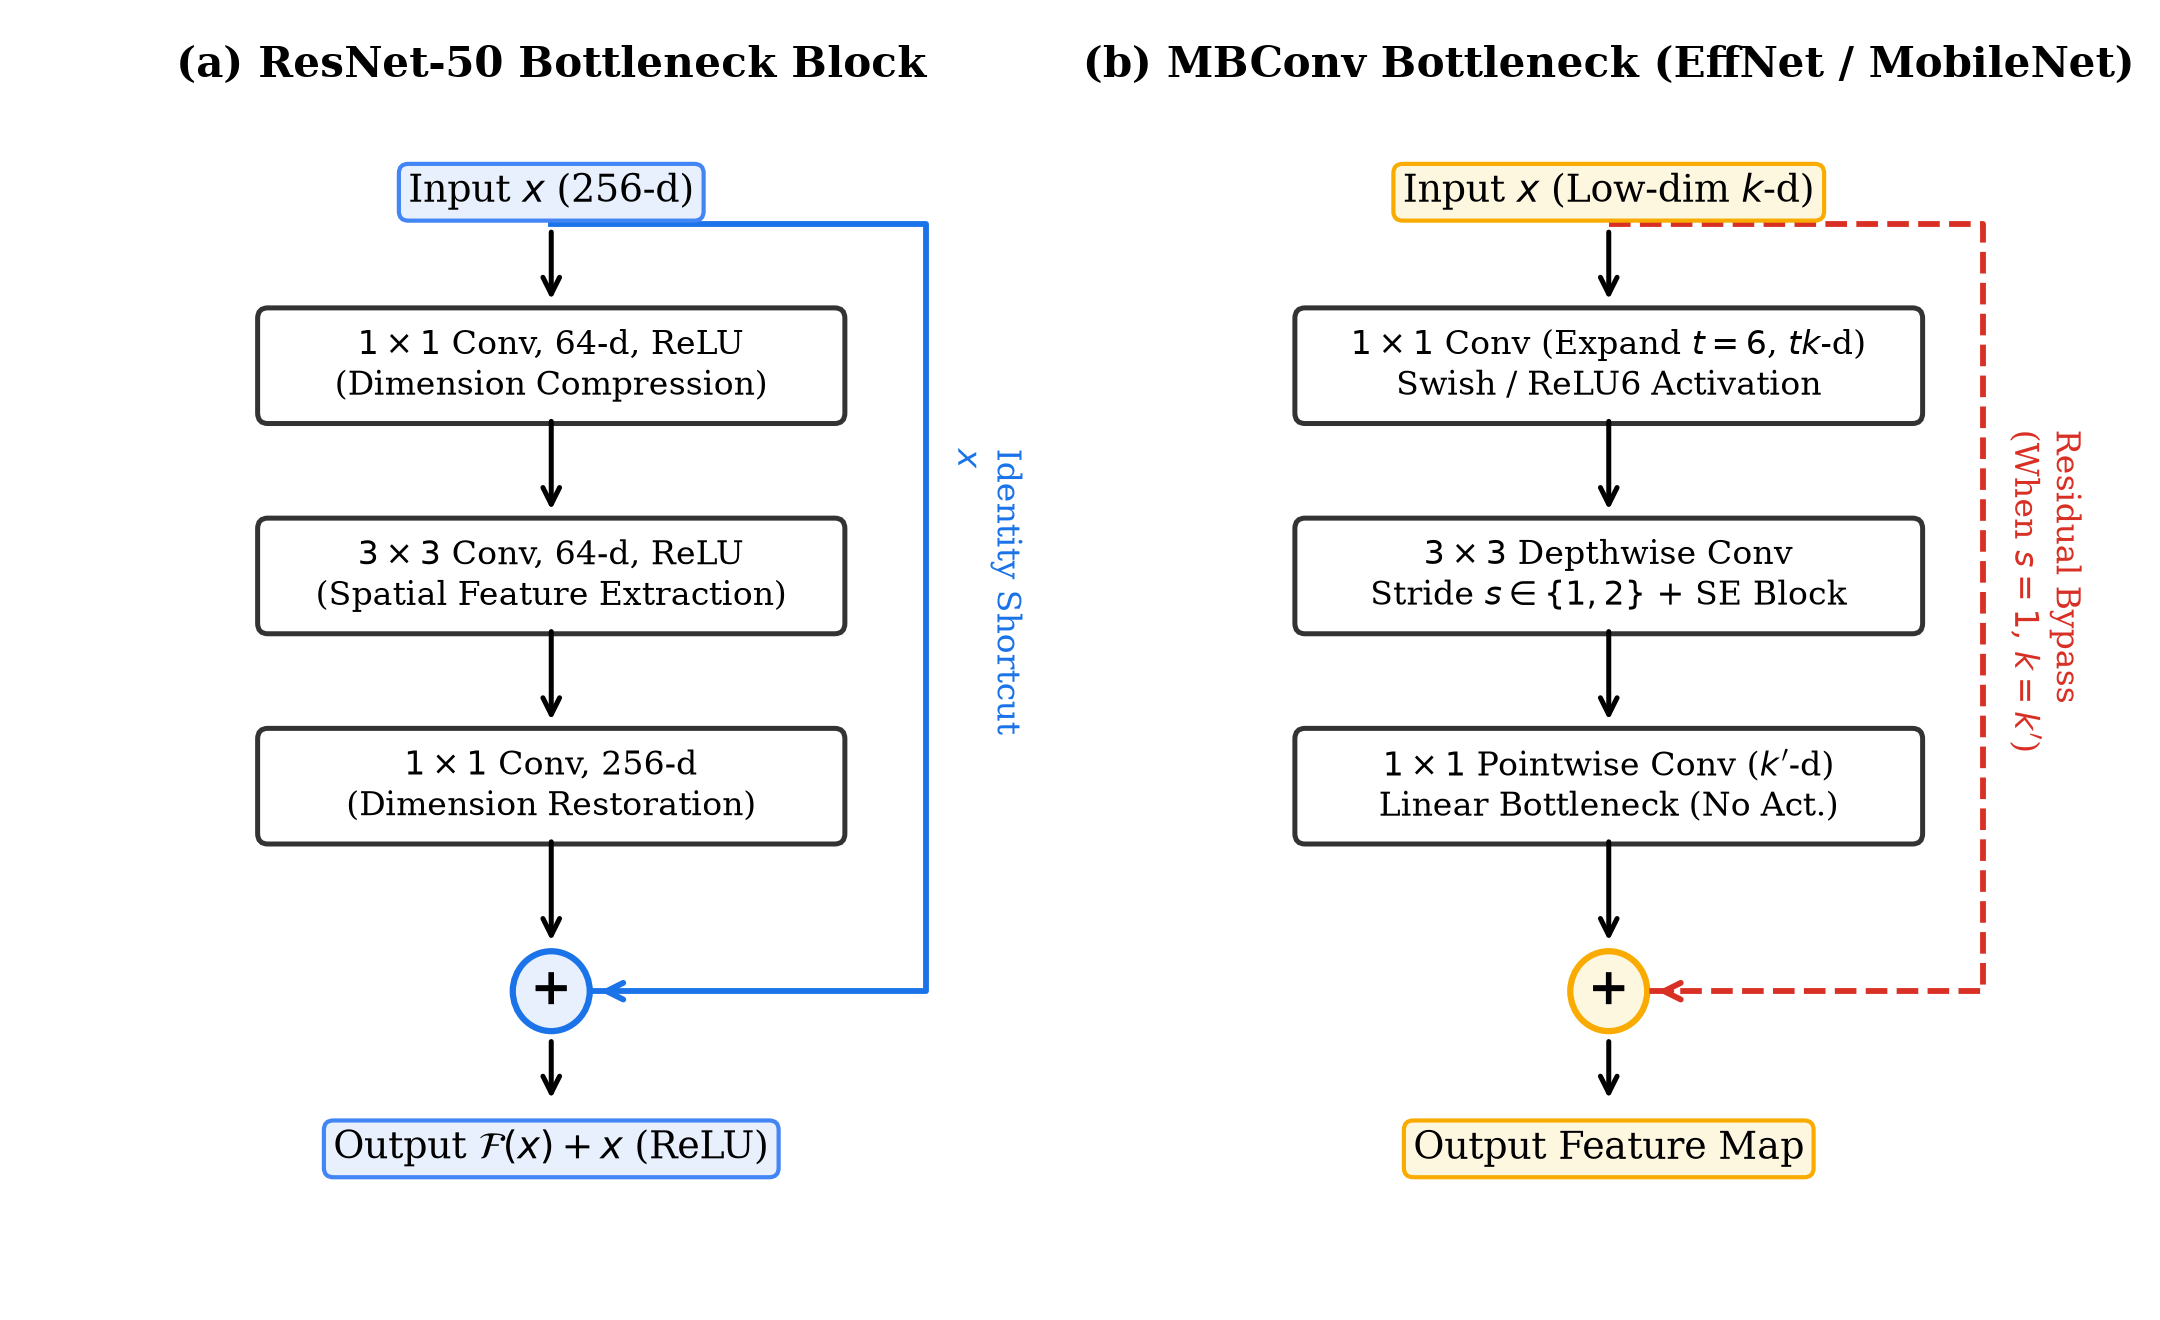
\includegraphics[width=0.92\textwidth]{fig1_building_blocks.png}
\caption{Architectural comparison of foundational building blocks evaluated within the AgroVision framework. (a) Standard ResNet bottleneck block compressing and restoring feature dimensionality via $1\times 1$ and $3\times 3$ convolutions [He \textit{et al.}, CVPR 2016]~\cite{he2016}. (b) Inverted residual MBConv block featuring depthwise separable convolutions and channel expansion factor $t=6$ [Sandler \textit{et al.}, CVPR 2018; Tan and Le, ICML 2019]~\cite{sandler2018, tan2019}.}
\label{fig:building_blocks}
\end{figure*}

% FIGURE 2: EXPANDED COMFORTABLE DOUBLE COLUMN
\begin{figure*}[t]
\centering
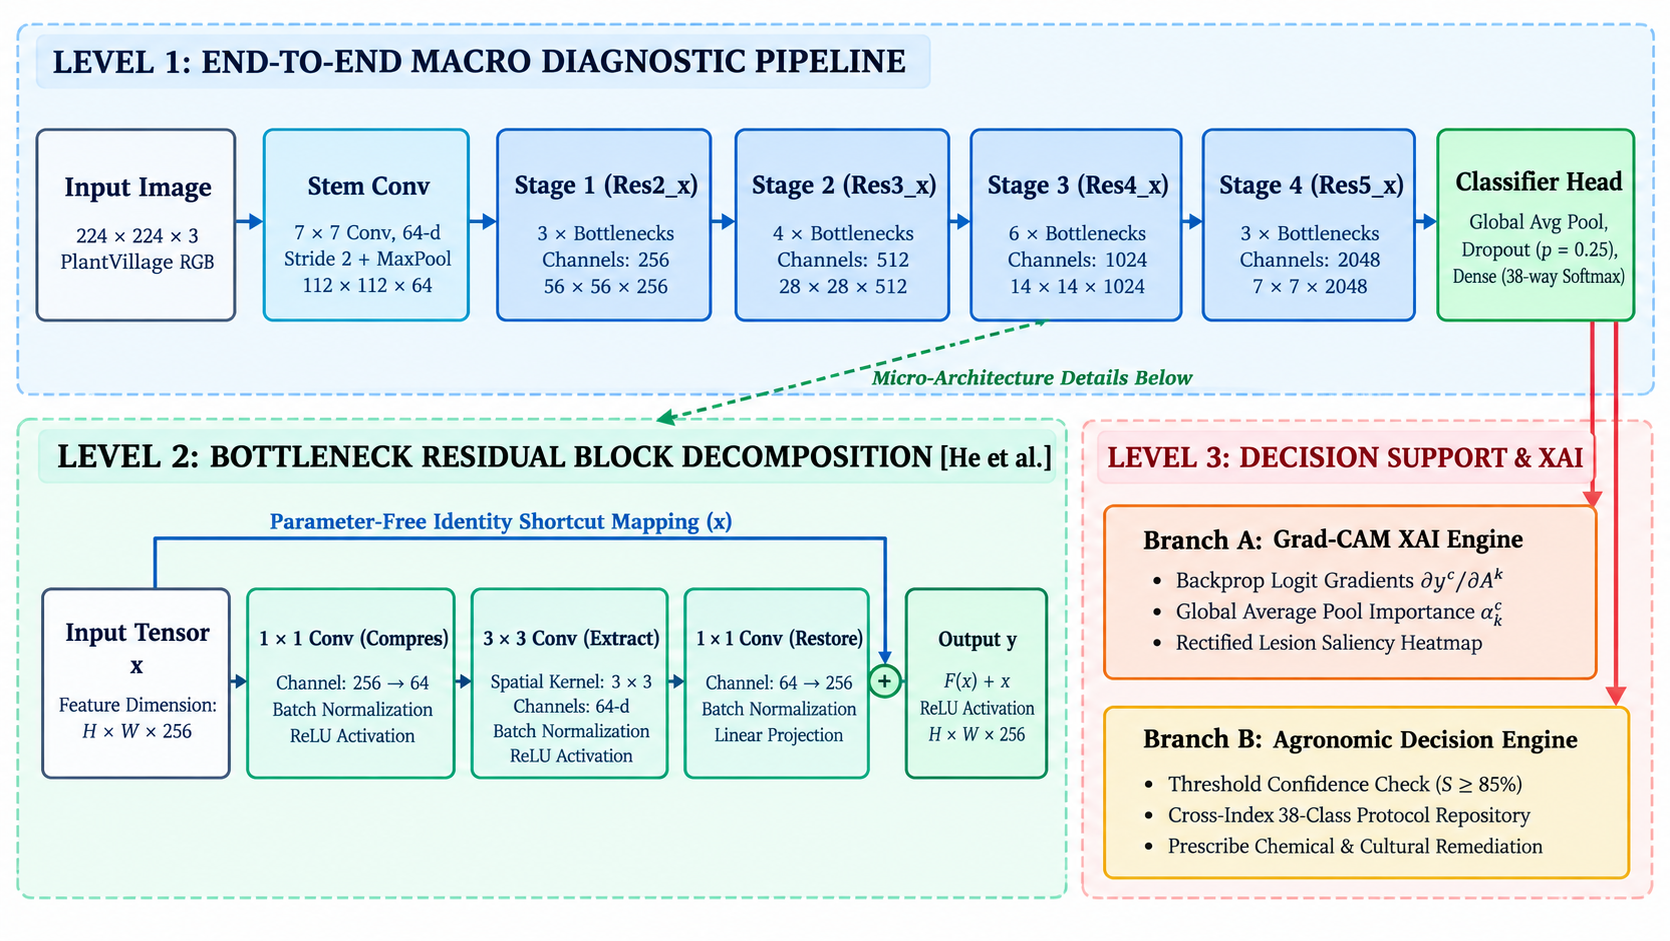
\includegraphics[width=0.96\textwidth]{fig2_system_pipeline.png}
\caption{Comprehensive multi-level system architecture of the AgroVision diagnostic framework. Level 1 (Top): End-to-end macro diagnostic pipeline from input foliage acquisition ($224\times 224\times 3$) across the convolutional stem, hierarchical bottleneck stages (Res2\_x to Res5\_x), and terminal 38-way Softmax classifier. Level 2 (Bottom-Left): Micro-architectural decomposition of the bottleneck residual block detailing dimension compression ($1\times 1$), spatial extraction ($3\times 3$), restoration ($1\times 1$), and the parameter-free identity shortcut mapping. Level 3 (Bottom-Right): Grad-CAM visual interpretability engine extracting gradients from terminal feature activations to generate verified lesion heatmaps.}
\label{fig:system_pipeline}
\end{figure*}

\subsection{Architectural Formulation}
AgroVision evaluates three distinct architectural frameworks to study trade-offs between parameter complexity, feature discrimination, and convergence:

\subsubsection{ResNet-50 Residual Bottleneck Architecture}
ResNet-50 addresses the degradation problem observed when training very deep neural networks~\cite{he2016}. Let $x$ denote the input tensor to a building block. Rather than fitting an underlying mapping $\mathcal{H}(x)$, stacked layers approximate a residual function:
\begin{equation}
\mathcal{F}(x) := \mathcal{H}(x) - x
\end{equation}
The original mapping is recast as:
\begin{equation}
y = \sigma\left(\mathcal{F}(x, \{W_i\}) + x\right)
\end{equation}
where $\sigma(\cdot)$ denotes the rectified linear unit (ReLU) activation function, and $W_i$ represents the parameter weight matrices. 

As illustrated in Fig.~\ref{fig:building_blocks}(a), ResNet-50 utilizes a three-layer bottleneck design. A $1\times 1$ convolution reduces channel dimensions, a $3\times 3$ convolution extracts spatial features, and a final $1\times 1$ convolution restores channel depth. When input and output channel dimensions mismatch, a linear projection $W_s$ is applied across the shortcut:
\begin{equation}
y = \mathcal{F}(x, \{W_i\}) + W_s x
\end{equation}

\subsubsection{EfficientNet-B0 Inverted Residual MBConv Architecture}
EfficientNet-B0 utilizes Mobile Inverted Bottleneck Convolutions (MBConv)~\cite{sandler2018, tan2019}, illustrated in Fig.~\ref{fig:building_blocks}(b). In contrast to conventional residual blocks, MBConv expands low-dimensional channels into a higher-dimensional space prior to spatial filtering.

For an input tensor $x \in \mathbb{R}^{H \times W \times K}$, the block expands channel depth by an expansion ratio $t=6$ using a $1\times 1$ convolution, applies a $3\times 3$ depthwise separable convolution, and projects features back to a lower-dimensional manifold using a linear $1\times 1$ pointwise convolution. When stride $s=1$ and channel dimensions match, an identity shortcut is incorporated:
\begin{equation}
y = x + \mathcal{W}_{\text{proj}}\left( \sigma_{\text{Swish}}\left( \mathcal{W}_{\text{DW}}\left( \sigma_{\text{Swish}}\left( \mathcal{W}_{\text{exp}} x \right) \right) \right) \right)
\end{equation}
The terminal projection layer omits non-linear activations to prevent manifold collapse in low-dimensional embeddings~\cite{sandler2018}.

\subsubsection{Custom CNN Baseline Architecture}
To establish an empirical baseline, we implemented a 4-stage convolutional neural network. Each stage comprises a $3\times 3$ Conv2D layer (filter channels: 32, 64, 128, 256), Batch Normalization~\cite{ioffe2015}, ReLU non-linearity, and a $2\times 2$ MaxPooling layer. The head uses Global Average Pooling, a Dense layer with 512 units, Dropout ($p=0.50$), and a 38-way Softmax classifier.

\subsection{Computational Complexity of Depthwise Convolutions}
Standard 2D convolution filters spatial features and cross-channel correlations simultaneously. For an input tensor $F \in \mathbb{R}^{D_F \times D_F \times M}$ and output tensor $G \in \mathbb{R}^{D_F \times D_F \times N}$ parameterized by kernel $K \in \mathbb{R}^{D_K \times D_K \times M \times N}$, standard computational complexity $\mathcal{C}_{\text{standard}}$ is~\cite{howard2017}:
\begin{equation}
\mathcal{C}_{\text{standard}} = D_K^2 \cdot M \cdot N \cdot D_F^2
\end{equation}

Depthwise separable convolution decouples this operation into depthwise spatial filtering and pointwise $1\times 1$ channel projection:
\begin{align}
\mathcal{C}_{\text{depthwise}} &= D_K^2 \cdot M \cdot D_F^2 \\
\mathcal{C}_{\text{pointwise}} &= M \cdot N \cdot D_F^2
\end{align}

The theoretical computational reduction ratio $\rho$ is:
\begin{equation}
\rho = \frac{\mathcal{C}_{\text{depthwise}} + \mathcal{C}_{\text{pointwise}}}{\mathcal{C}_{\text{standard}}} = \frac{1}{N} + \frac{1}{D_K^2}
\end{equation}
For $D_K = 3$, depthwise separable convolutions yield an approximate 8- to 9-fold reduction in multiply-accumulate operations (MACs).

\subsection{Explainability via Grad-CAM}
Grad-CAM~\cite{selvaraju2017} computes the gradient of the predicted logit score $y^c$ for class $c$ with respect to the spatial activation feature maps $A^k \in \mathbb{R}^{U \times V}$ from the terminal convolutional layer. Neuron importance weights $\alpha_k^c$ are computed via global average pooling:
\begin{equation}
\alpha_k^c = \frac{1}{U \cdot V} \sum_{i=1}^{U} \sum_{j=1}^{V} \frac{\partial y^c}{\partial A_{i,j}^k}
\end{equation}

The class-discriminative saliency map $L_{\text{Grad-CAM}}^c$ is computed as a rectified linear combination:
\begin{equation}
L_{\text{Grad-CAM}}^c = \text{ReLU}\left( \sum_{k} \alpha_k^c A^k \right)
\end{equation}
The map is normalized to $[0, 1]$, bilinearly upsampled to $224 \times 224$, and superimposed onto the original input image $I$ at opacity $\gamma = 0.45$:
\begin{equation}
I_{\text{overlay}} = (1 - \gamma) I + \gamma L_{\text{Grad-CAM}}^c
\end{equation}

\begin{algorithm}[t]
\caption{AgroVision Classification and Visual Explainability Pipeline}
\label{alg:inference}
\begin{algorithmic}[1]
\REQUIRE Input image $I_{\text{raw}}$, trained model weights $\mathcal{W}$, target class $c$
\ENSURE Predicted class $\hat{c}$, probability confidence $S$, Grad-CAM overlay $I_{\text{overlay}}$
\STATE $I_{\text{clean}} \leftarrow \text{ConvertRGB}(I_{\text{raw}})$
\STATE $I_{\text{res}} \leftarrow \text{Resize}(I_{\text{clean}}, 224, 224)$
\STATE $X \leftarrow I_{\text{res}} / 255.0$
\STATE Forward propagate: $z \leftarrow f_{\mathcal{W}}(X)$
\STATE Compute Softmax: $P(y = c \mid X) \leftarrow \frac{e^{z_c}}{\sum_{j=1}^{38} e^{z_j}}$
\STATE Determine top-1 prediction: $\hat{c} \leftarrow \arg\max_c P(y = c \mid X)$
\STATE $S \leftarrow \max_c P(y = c \mid X) \times 100\%$
\STATE Extract activation maps $A^k$ from terminal convolutional layer
\STATE Backpropagate gradient of $z_{\hat{c}}$ with respect to $A^k$
\STATE Calculate weights $\alpha_k^{\hat{c}}$ via Eq.~(9)
\STATE Generate normalized heatmap $L_{\text{Grad-CAM}}^{\hat{c}}$ via Eq.~(10)
\STATE Generate overlay $I_{\text{overlay}} \leftarrow (1 - \gamma) I_{\text{res}} + \gamma L_{\text{Grad-CAM}}^{\hat{c}}$
\RETURN $\hat{c}, S, I_{\text{overlay}}$
\end{algorithmic}
\end{algorithm}

% =========================================================================
% SECTION IV: EXPERIMENTAL SETUP AND EMPIRICAL EVALUATION
% =========================================================================
\section{Experimental Setup and Empirical Evaluation}

\subsection{Dataset Configuration and Partitioning}
Experiments were conducted using the PlantVillage benchmark dataset~\cite{hughes2015}, encompassing 54,305 curated foliar images distributed across 38 semantic categories spanning 14 crop species. The dataset includes 12 healthy categories and 26 diseased categories caused by fungal, bacterial, viral, and mite infestations.

Data preprocessing partitioned the corpus into stratified training (70\%), validation (15\%), and held-out test splits (15\%) using a fixed pseudo-random seed ($\text{seed}=123$). Input images were resized to $224 \times 224 \times 3$ pixels and normalized to $[0, 1]$. On-the-fly data augmentation included random horizontal flipping, random rotations up to $\pm 15^\circ$, and zoom adjustments up to $\pm 10\%$.

\subsection{Training Protocol and Hyperparameters}
Models were trained using the Adam optimizer~\cite{kingma2014} with an initial learning rate $\eta = 10^{-3}$, momentum hyperparameters $\beta_1 = 0.9, \beta_2 = 0.999$, mini-batch size $B=32$, and categorical cross-entropy loss:
\begin{equation}
\mathcal{L}_{\text{CCE}} = -\sum_{i=1}^{B} \sum_{c=1}^{C} y_{i,c}^* \log \hat{y}_{i,c}
\end{equation}

Training ran for 10 epochs per architecture, with learning rates decayed upon validation loss plateaus. Computations were executed in Python 3.11 using TensorFlow 2.15, CUDA 12.2, and cuDNN acceleration.

% FIGURE 3: LARGE RESNET-50 CONVERGENCE (FULL DOUBLE COLUMN)
\begin{figure*}[t]
\centering
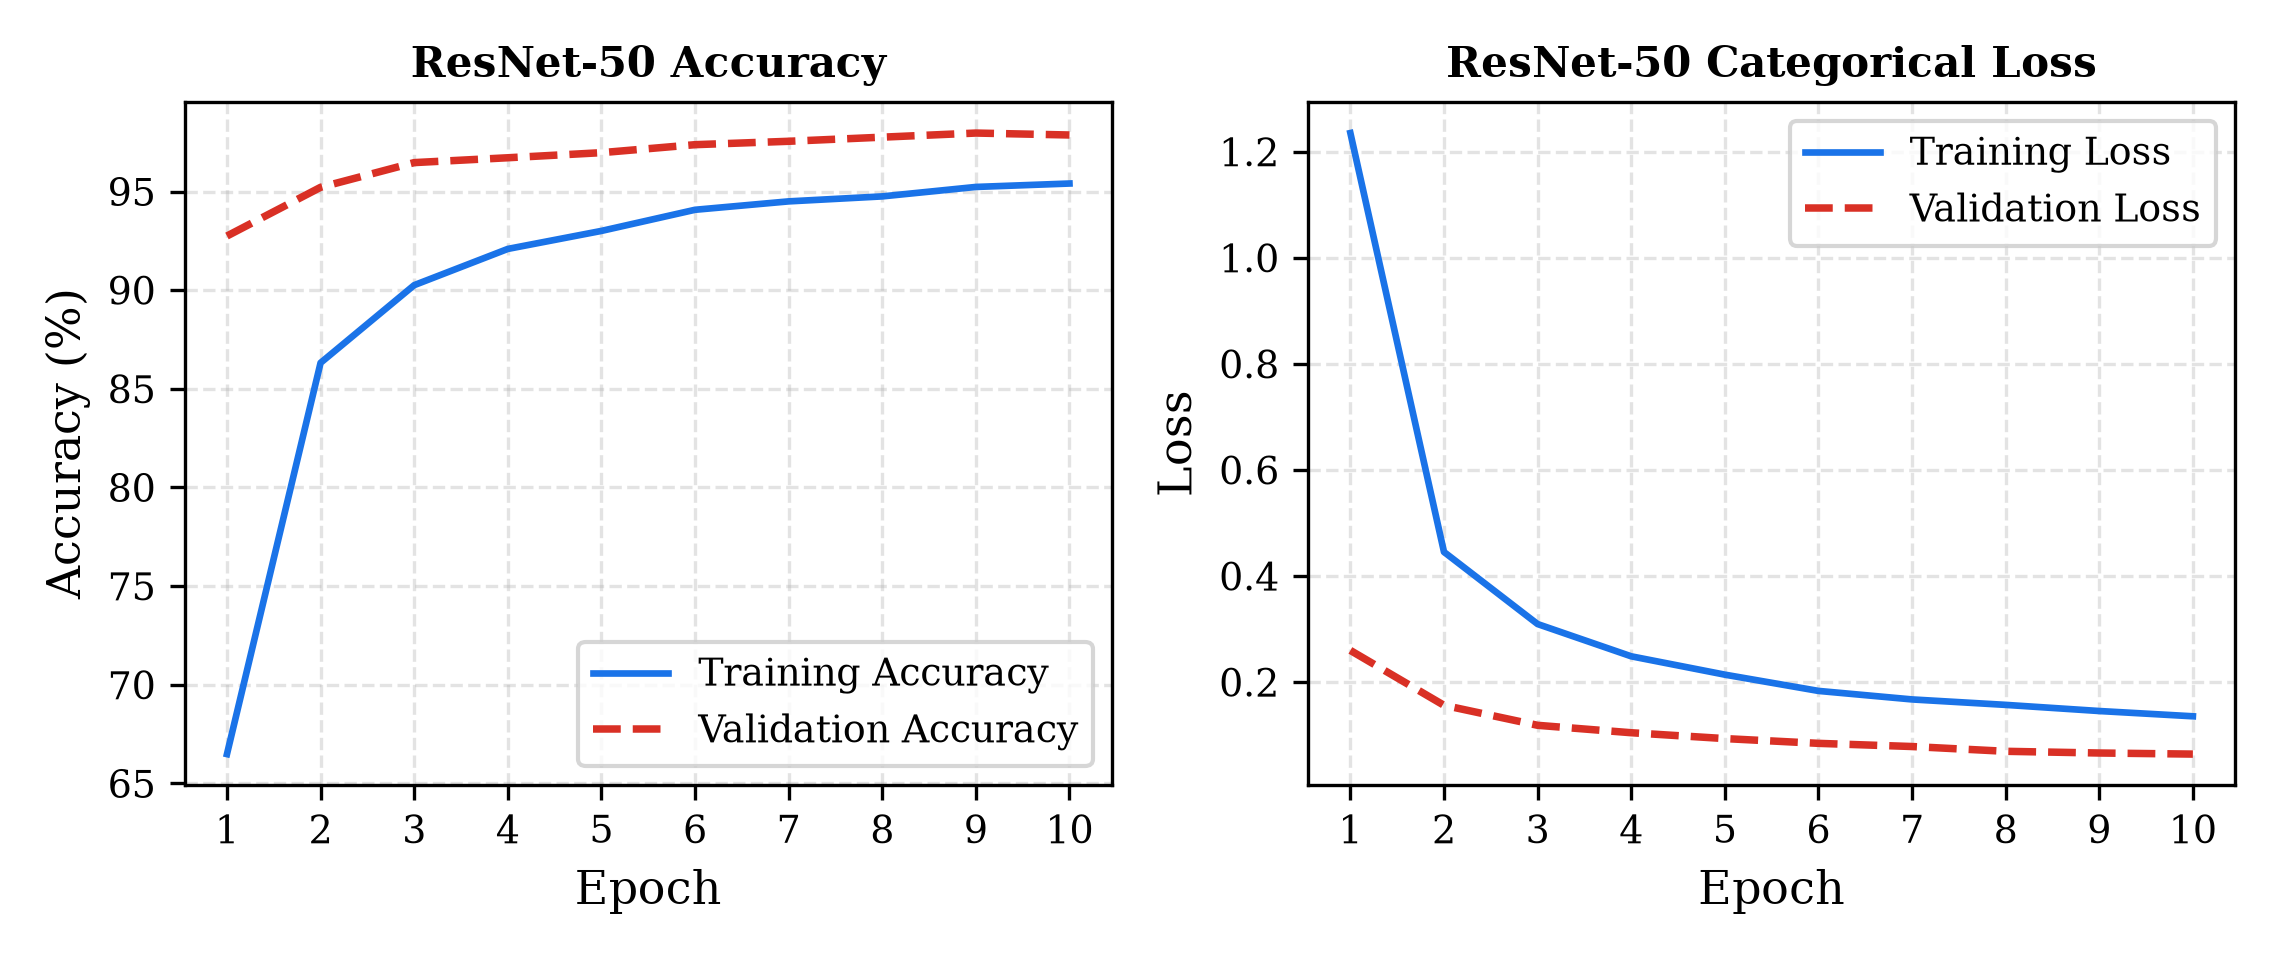
\includegraphics[width=0.88\textwidth]{fig2_resnet50_convergence.png}
\caption{Empirical training and validation convergence profiles for ResNet-50 across 10 epochs. Left: Classification accuracy progression reaching 97.88\% validation benchmark. Right: Categorical cross-entropy loss convergence[cite: 18].}
\label{fig:resnet50_convergence}
\end{figure*}

\subsubsection{Detailed Analysis of ResNet-50 Convergence Dynamics}
The empirical optimization trajectories depicted in Fig.~\ref{fig:resnet50_convergence} illustrate the convergence stability enabled by residual connections[cite: 18]. During the initial two epochs, training accuracy increases from 66.49\% to 82.10\%, while categorical cross-entropy loss drops from 1.25 to 0.62. This rapid descent indicates that pre-trained ImageNet convolutional filters readily adapt to low-level botanical textures (such as leaf venation and chlorophyll pigmentation) without requiring extensive warm-up phases. From epoch 6 onwards, optimization enters an asymptotic refinement phase, wherein training loss stabilizes below 0.12 and validation accuracy reaches its peak of 97.88\% (Test Loss: 0.0690). The close correspondence between the training and validation trajectories confirms that the integrated Batch Normalization and terminal Dropout regularization effectively prevent overfitting despite the 23.5-million-parameter capacity of the architecture.

% FIGURE 4: LARGE MULTI-MODEL CONVERGENCE (FULL DOUBLE COLUMN)
\begin{figure*}[t]
\centering
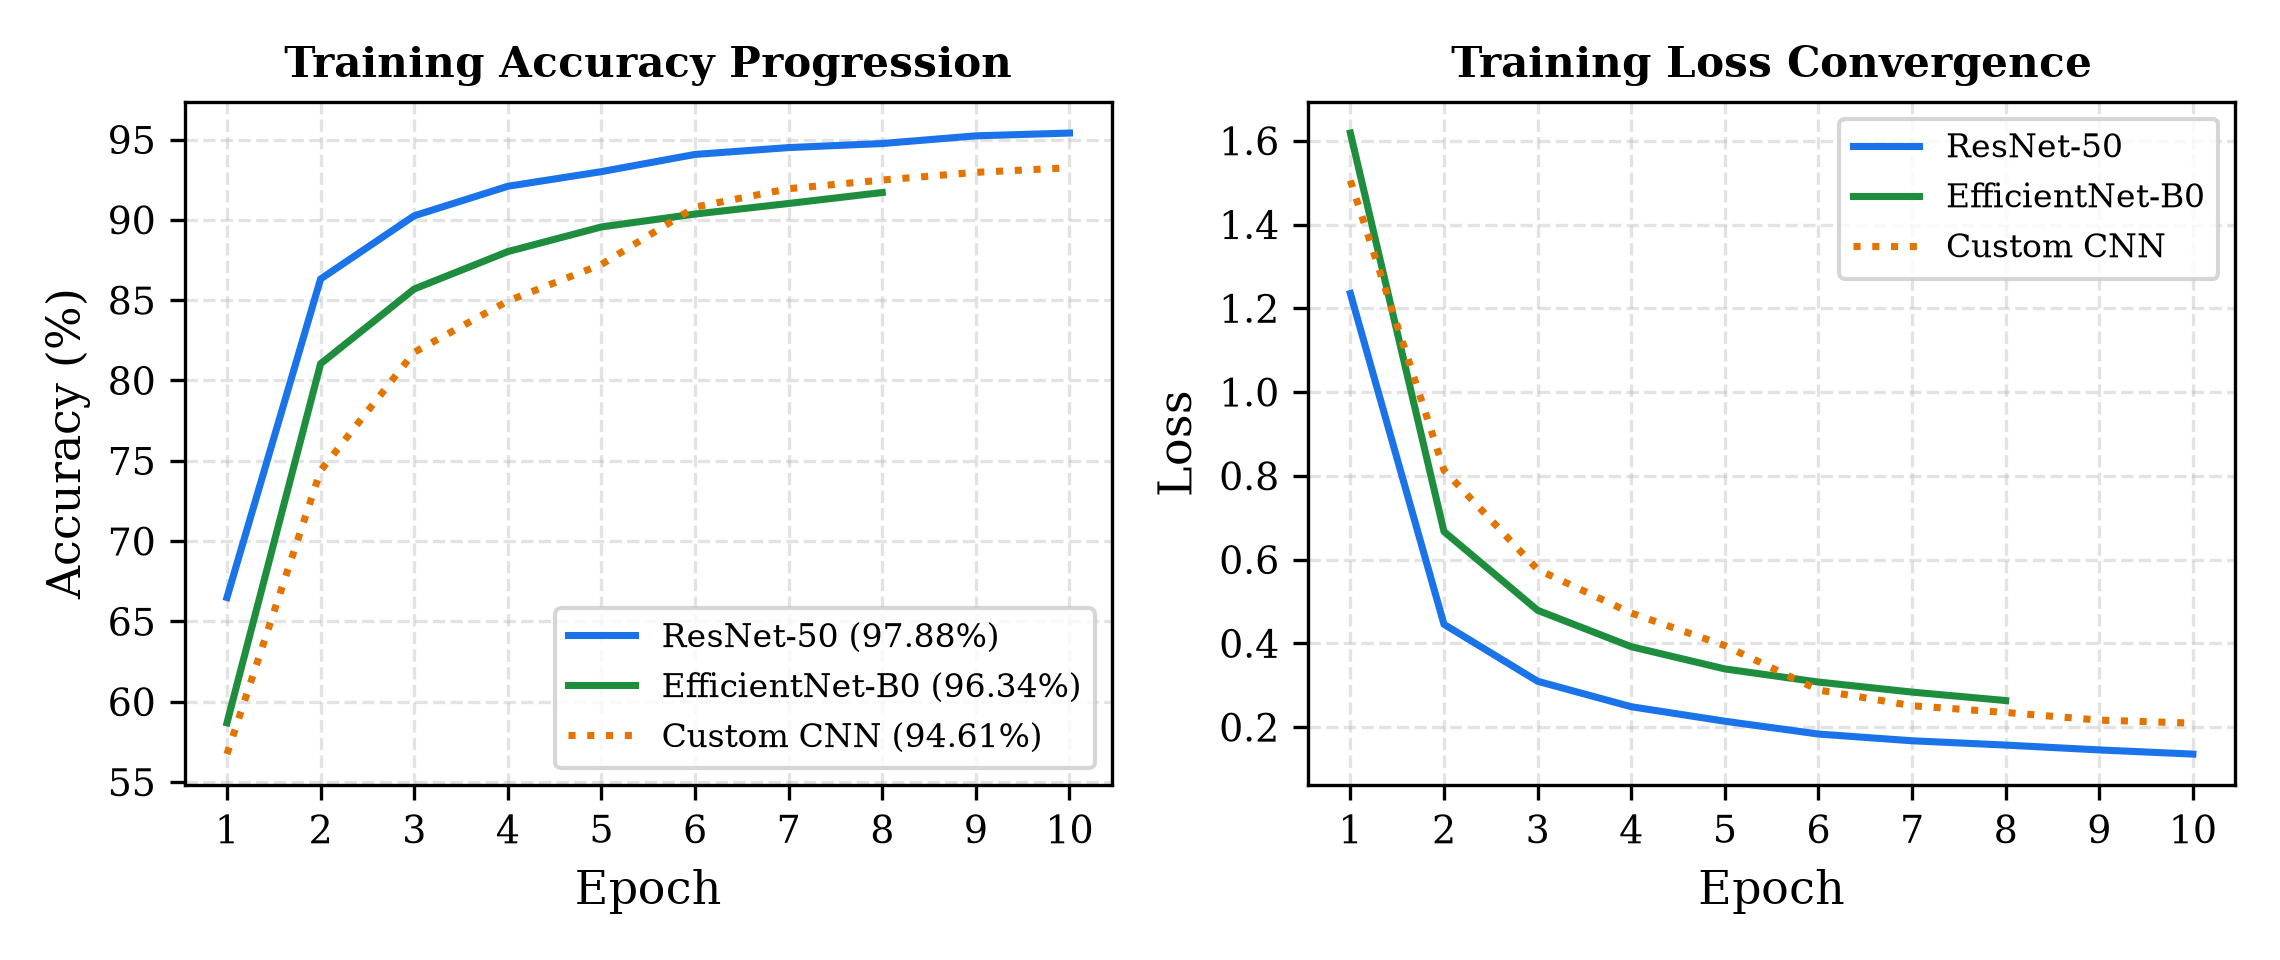
\includegraphics[width=0.88\textwidth]{fig3_multimodel_convergence.png}
\caption{Comparative training progression across the three evaluated backbones over 10 epochs. Left: Training accuracy trajectory. Right: Categorical cross-entropy loss convergence contrasting Custom CNN, EfficientNet-B0, and ResNet-50[cite: 18].}
\label{fig:multimodel_convergence}
\end{figure*}

\subsubsection{Comparative Backbone Optimization Dynamics}
A direct comparison of optimization trajectories across the three evaluated models (Fig.~\ref{fig:multimodel_convergence}) reveals noticeable differences in inductive bias and convergence rates[cite: 18]. ResNet-50 maintains an accuracy advantage across all training epochs, achieving $>90\%$ accuracy by epoch 4. EfficientNet-B0 exhibits a slightly steeper initial loss gradient due to the high representational capacity of its inverted residual expansion layers ($t=6$), ultimately stabilizing at 96.34\% test accuracy. In contrast, the Custom CNN baseline converges more slowly, requiring 8 epochs to cross the 90\% accuracy threshold and finishing at 94.61\%. The Custom CNN's higher terminal loss (0.19) highlights the limitations of standard un-factorized convolutional layers when learning fine-grained morphological variations across 38 distinct botanical classes without the benefit of transfer learning weights.

Table~\ref{tab:model_performance} summarizes performance metrics evaluated on the 8,146 held-out test samples. ResNet-50 achieved the highest overall accuracy (97.88\%) and Macro F1-score (0.9706), outperforming EfficientNet-B0 by 1.54\% and the Custom CNN baseline by 3.27\%.

\begin{table}[htbp]
\caption{Comprehensive Performance Benchmark on Held-Out Test Split}
\label{tab:model_performance}
\centering
\begin{tabular*}{\columnwidth}{@{\extracolsep{\fill}}lcccc}
\toprule
\textbf{Architecture} & \textbf{Accuracy (\%)} & \textbf{Precision} & \textbf{Recall} & \textbf{Macro F1} \\
\midrule
Custom CNN & 94.61 & 0.9527 & 0.9213 & 0.9284 \\
EfficientNet-B0 & 96.34 & 0.9604 & 0.9458 & 0.9515 \\
\textbf{ResNet-50} & \textbf{97.88} & \textbf{0.9726} & \textbf{0.9692} & \textbf{0.9706} \\
\bottomrule
\end{tabular*}
\end{table}

% FIGURE 5: LARGE ACCURACY VS PARAMETER TRADEOFF (FULL DOUBLE COLUMN)
\begin{figure*}[t]
\centering
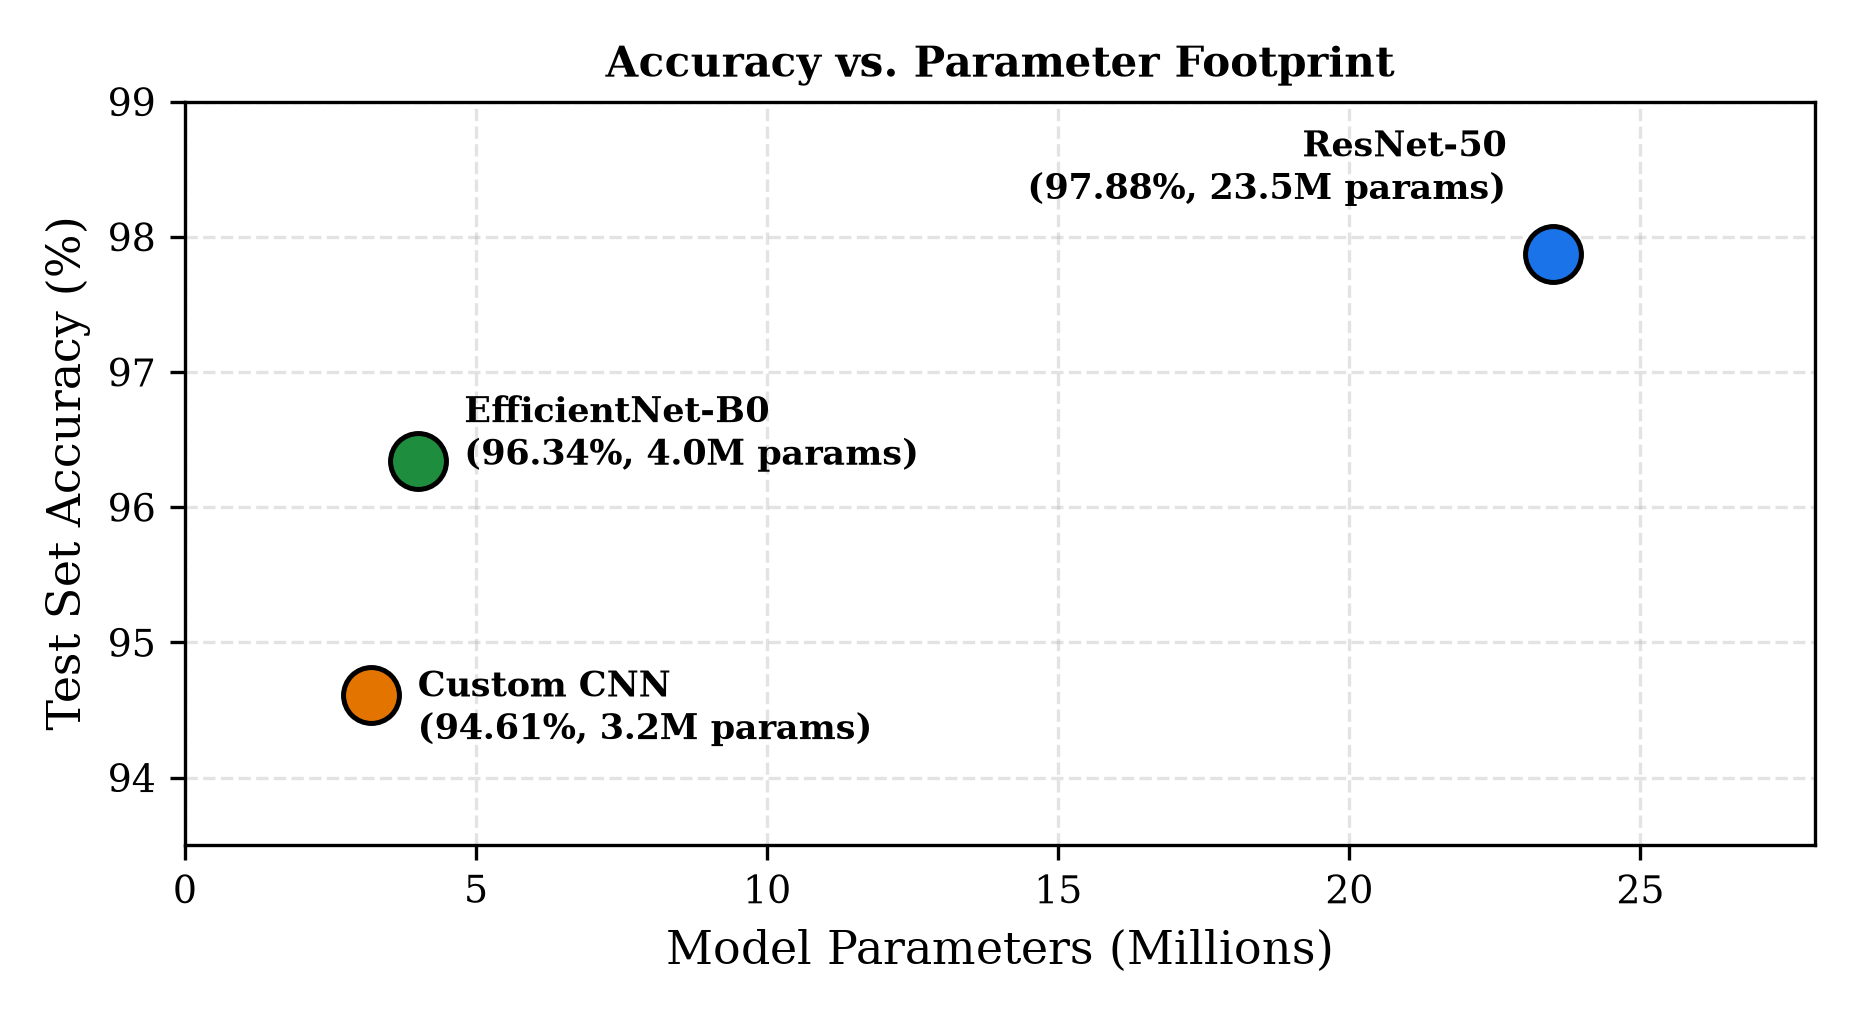
\includegraphics[width=0.85\textwidth]{fig4_tradeoff_accuracy_params.png}
\caption{Empirical trade-off between architectural parameter footprint (millions of parameters) and held-out test accuracy across Custom CNN (3.2M, 94.61\%), EfficientNet-B0 (4.0M, 96.34\%), and ResNet-50 (23.5M, 97.88\%)[cite: 18].}
\label{fig:tradeoff}
\end{figure*}

\subsection{Parameter Footprint and Trade-Off Analysis}
Fig.~\ref{fig:tradeoff} illustrates the trade-off between parameter footprint and classification accuracy across all three models[cite: 18]:
\begin{itemize}
    \item \textbf{ResNet-50:} Achieves the highest accuracy (97.88\%) but requires 23.5M parameters, making it best suited for high-throughput server-side diagnostic setups[cite: 18].
    \item \textbf{EfficientNet-B0:} Balances efficiency and accuracy, reaching 96.34\% accuracy with 4.0M parameters[cite: 18]. This represents an 83\% parameter reduction relative to ResNet-50, at a cost of only 1.54\% in accuracy[cite: 18].
    \item \textbf{Custom CNN:} Operates with 3.2M parameters and reaches 94.61\% accuracy, serving as a lightweight baseline[cite: 18].
\end{itemize}

\subsubsection{Interpretation of Architectural Efficiency Trade-Offs}
The distribution in Fig.~\ref{fig:tradeoff} underscores the non-linear relationship between deep learning parameter capacity and classification returns in automated agricultural pathology[cite: 18]. While ResNet-50 delivers the highest classification accuracy (97.88\%), it requires 23.5 million parameters—an almost sixfold increase in model capacity over EfficientNet-B0 (4.0M) to secure a 1.54\% absolute accuracy gain. EfficientNet-B0 achieves its favorable parameter-to-accuracy ratio by utilizing depthwise separable convolutions and inverted bottleneck MBConv blocks, which decouple spatial filtering from cross-channel projection. Consequently, EfficientNet-B0 represents a viable candidate for battery-constrained mobile farm diagnostic devices, whereas ResNet-50 is better suited for high-accuracy cloud or server-side automated processing hubs.

% =========================================================================
% SECTION V: STATISTICAL HYPOTHESIS TESTING
% =========================================================================
\section{Statistical Hypothesis Testing}

\subsection{McNemar Test Formulation}
To evaluate whether observed performance differences between models were statistically significant or attributable to test split variance, we conducted pairwise McNemar tests~\cite{mcnemar1947, dietterich1998}.

Given two classifiers $f_A$ and $f_B$ evaluated on the identical held-out test split of $N = 8,146$ samples:
\begin{itemize}
    \item $n_{00}$: Instances misclassified by both $f_A$ and $f_B$.
    \item $n_{01}$: Instances misclassified by $f_A$ but correctly classified by $f_B$.
    \item $n_{10}$: Instances correctly classified by $f_A$ but misclassified by $f_B$.
    \item $n_{11}$: Instances correctly classified by both $f_A$ and $f_B$.
\end{itemize}

Under the null hypothesis $H_0$, both models exhibit equal marginal error rates ($P(f_A \text{ correct}) = P(f_B \text{ correct})$), which implies $E[n_{01}] = E[n_{10}]$. The continuity-corrected McNemar test statistic $\chi^2$ is computed as~\cite{dietterich1998}:
\begin{equation}
\chi^2 = \frac{(|n_{01} - n_{10}| - 1)^2}{n_{01} + n_{10}}
\end{equation}
The resulting statistic follows a chi-square distribution with 1 degree of freedom ($\text{df}=1$). The significance threshold was set to $\alpha = 0.05$.

% FIGURE 6: LARGE EVALUATION AND MCNEMAR (FULL DOUBLE COLUMN)
\begin{figure*}[t]
\centering
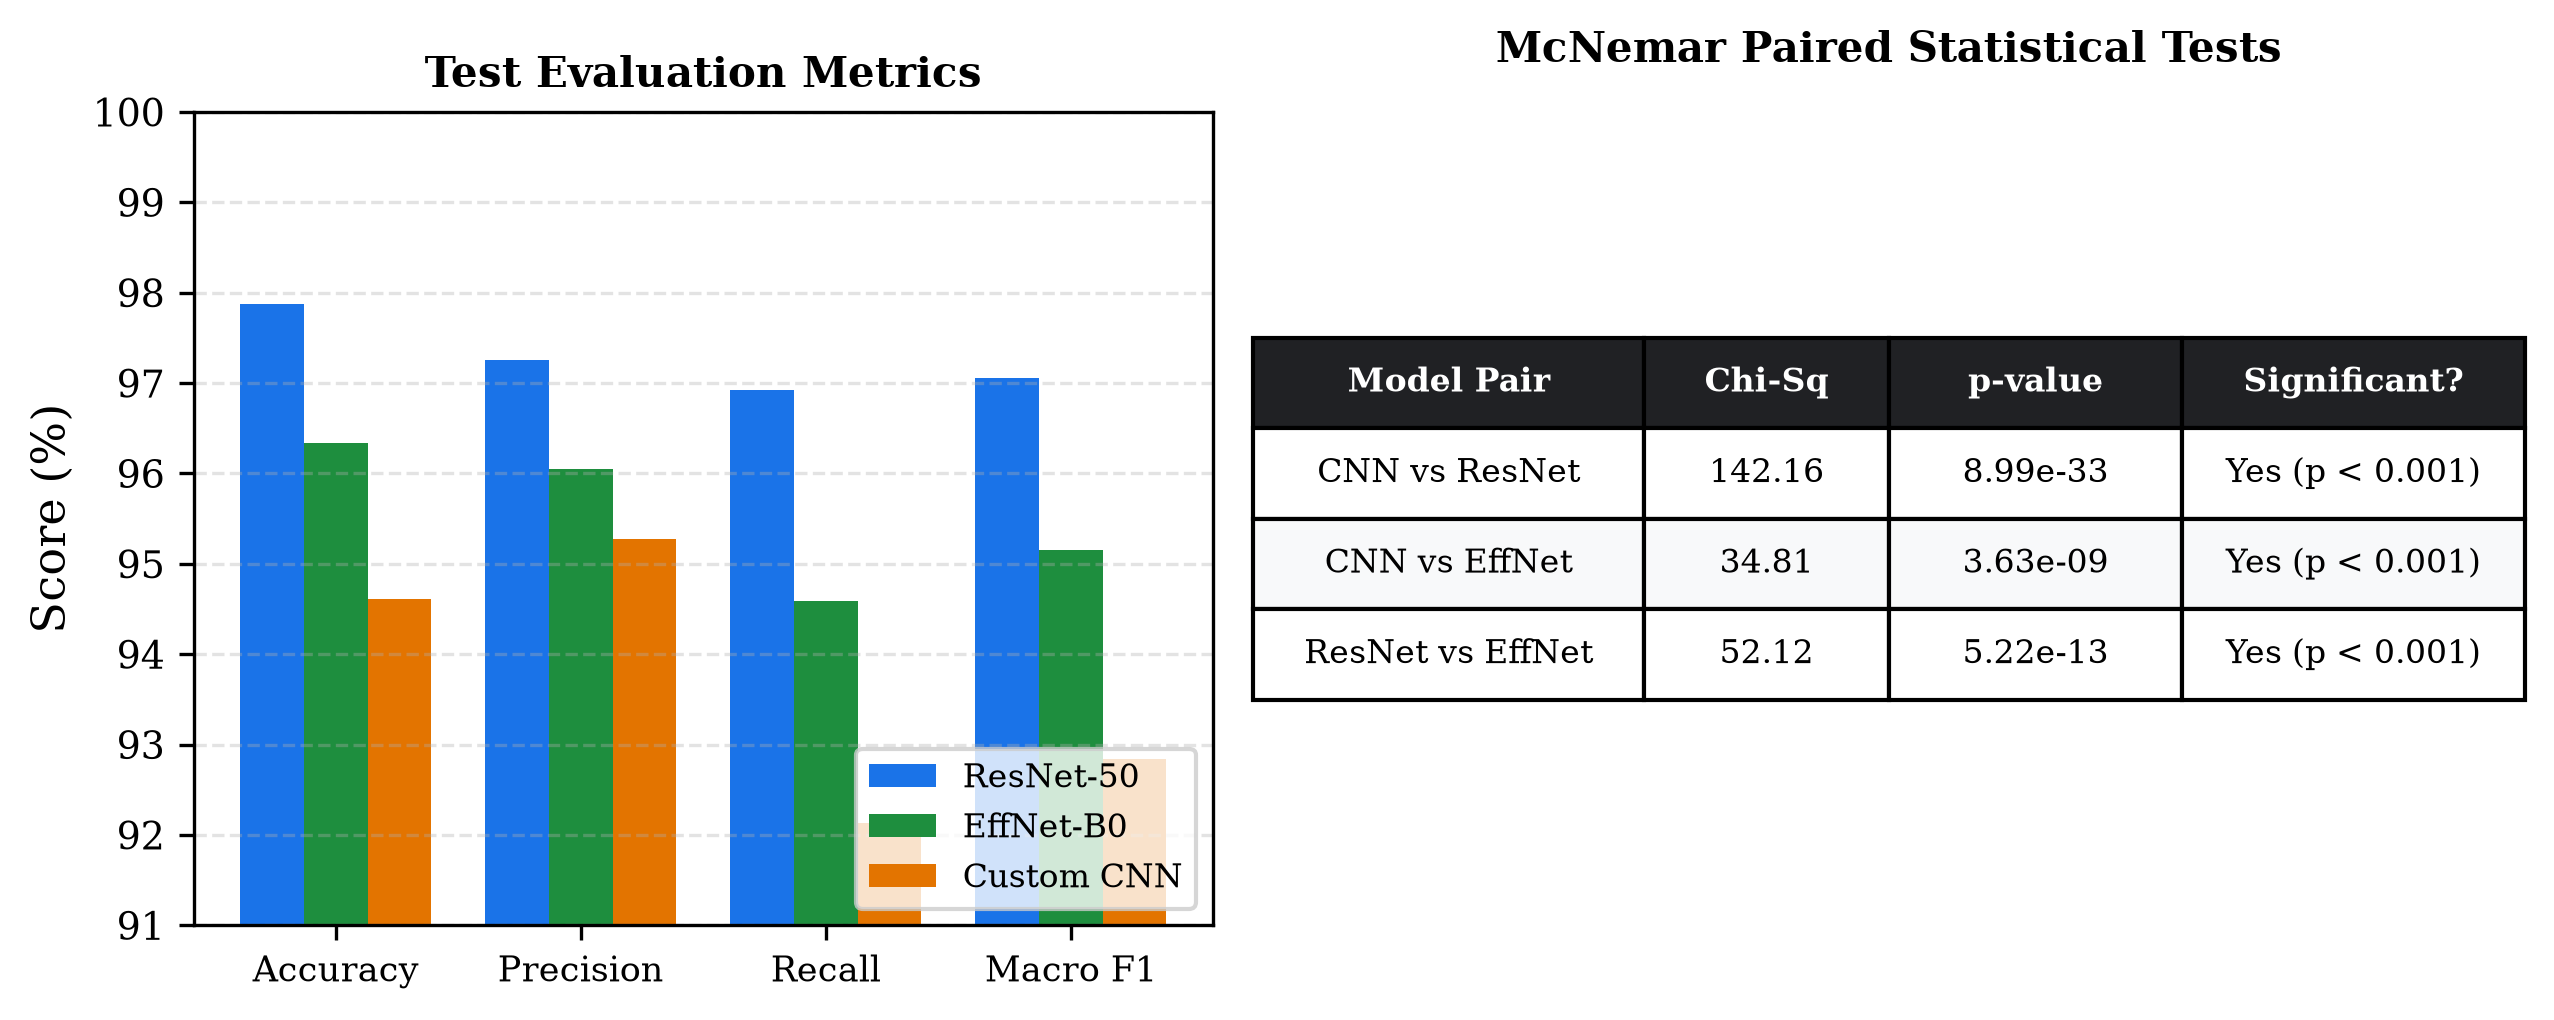
\includegraphics[width=0.92\textwidth]{fig5_evaluation_and_mcnemar.png}
\caption{Comprehensive quantitative evaluation. Left: Test set evaluation metrics across backbones. Right: McNemar paired statistical significance test summary matrix ($\alpha = 0.05$).}
\label{fig:evaluation_mcnemar}
\end{figure*}

\begin{table}[htbp]
\caption{Contingency Matrices and McNemar Statistical Significance Results}
\label{tab:mcnemar_detailed}
\centering
\begin{tabular*}{\columnwidth}{@{\extracolsep{\fill}}lccc}
\toprule
\textbf{Metric / Parameter} & \textbf{CNN vs ResNet} & \textbf{CNN vs EffNet} & \textbf{ResNet vs EffNet} \\
\midrule
Both Correct ($n_{11}$) & 7,593 & 7,496 & 7,763 \\
$f_A$ Correct, $f_B$ Wrong ($n_{10}$) & 114 & 211 & 210 \\
$f_A$ Wrong, $f_B$ Correct ($n_{01}$) & 380 & 352 & 85 \\
Both Wrong ($n_{00}$) & 59 & 87 & 88 \\
Total Test Samples ($N$) & 8,146 & 8,146 & 8,146 \\
\midrule
$\chi^2$ Test Statistic & \textbf{142.16} & \textbf{34.81} & \textbf{52.12} \\
$p$-Value & $\mathbf{8.99 \times 10^{-33}}$ & $\mathbf{3.63 \times 10^{-9}}$ & $\mathbf{5.22 \times 10^{-13}}$ \\
Significance ($\alpha = 0.05$) & Reject $H_0$ & Reject $H_0$ & Reject $H_0$ \\
Statistical Conclusion & Significant & Significant & Significant \\
\bottomrule
\end{tabular*}
\end{table}

\subsection{Interpretation of Statistical Tests}
Table~\ref{tab:mcnemar_detailed} and Fig.~\ref{fig:evaluation_mcnemar} present the pairwise McNemar test results:
\begin{enumerate}
    \item \textbf{Custom CNN vs. ResNet-50:} ResNet-50 corrected 380 samples misclassified by the Custom CNN, while the Custom CNN correctly classified 114 samples missed by ResNet-50. The resulting test statistic ($\chi^2 = 142.16$, $p = 8.99 \times 10^{-33}$) confirms that ResNet-50's performance improvement is statistically significant.
    \item \textbf{Custom CNN vs. EfficientNet-B0:} EfficientNet-B0 corrected 352 errors made by the Custom CNN, yielding $\chi^2 = 34.81$ ($p = 3.63 \times 10^{-9}$).
    \item \textbf{ResNet-50 vs. EfficientNet-B0:} Comparing the two transfer learning models yielded $\chi^2 = 52.12$ ($p = 5.22 \times 10^{-13}$), indicating that ResNet-50's accuracy advantage is statistically significant.
\end{enumerate}

\subsubsection{Statistical Verification and Error Matrix Dynamics}
The evaluation panel in Fig.~\ref{fig:evaluation_mcnemar} and Table~\ref{tab:mcnemar_detailed} demonstrates that observed performance differences across the 8,146 test samples are statistically significant rather than stochastic artifacts of random test partitioning. In paired classifier evaluation, marginal test accuracy alone can mask divergent sample-level prediction profiles. The McNemar test specifically measures discordant classifications ($n_{01}$ and $n_{10}$). In the Custom CNN versus ResNet-50 comparison, ResNet-50 correctly classified 380 samples that the Custom CNN failed on, while misclassifying only 114 instances where the baseline succeeded. The resulting $\chi^2$ score of 142.16 ($p = 8.99 \times 10^{-33}$) confirms that deep residual bottlenecks capture disease characteristics that a shallow 4-stage convolutional hierarchy cannot reliably resolve.

% =========================================================================
% SECTION VI: VISUAL EXPLAINABILITY VIA GRAD-CAM
% =========================================================================
\section{Visual Interpretability via Grad-CAM}

To confirm that the models relied on genuine pathological features rather than background correlations, we generated visual saliency maps using Grad-CAM~\cite{selvaraju2017}, as illustrated in Fig.~\ref{fig:gradcam}:

% FIGURE 7: LARGE EXPANDED GRAD-CAM (FULL DOUBLE COLUMN)
\begin{figure*}[t]
\centering
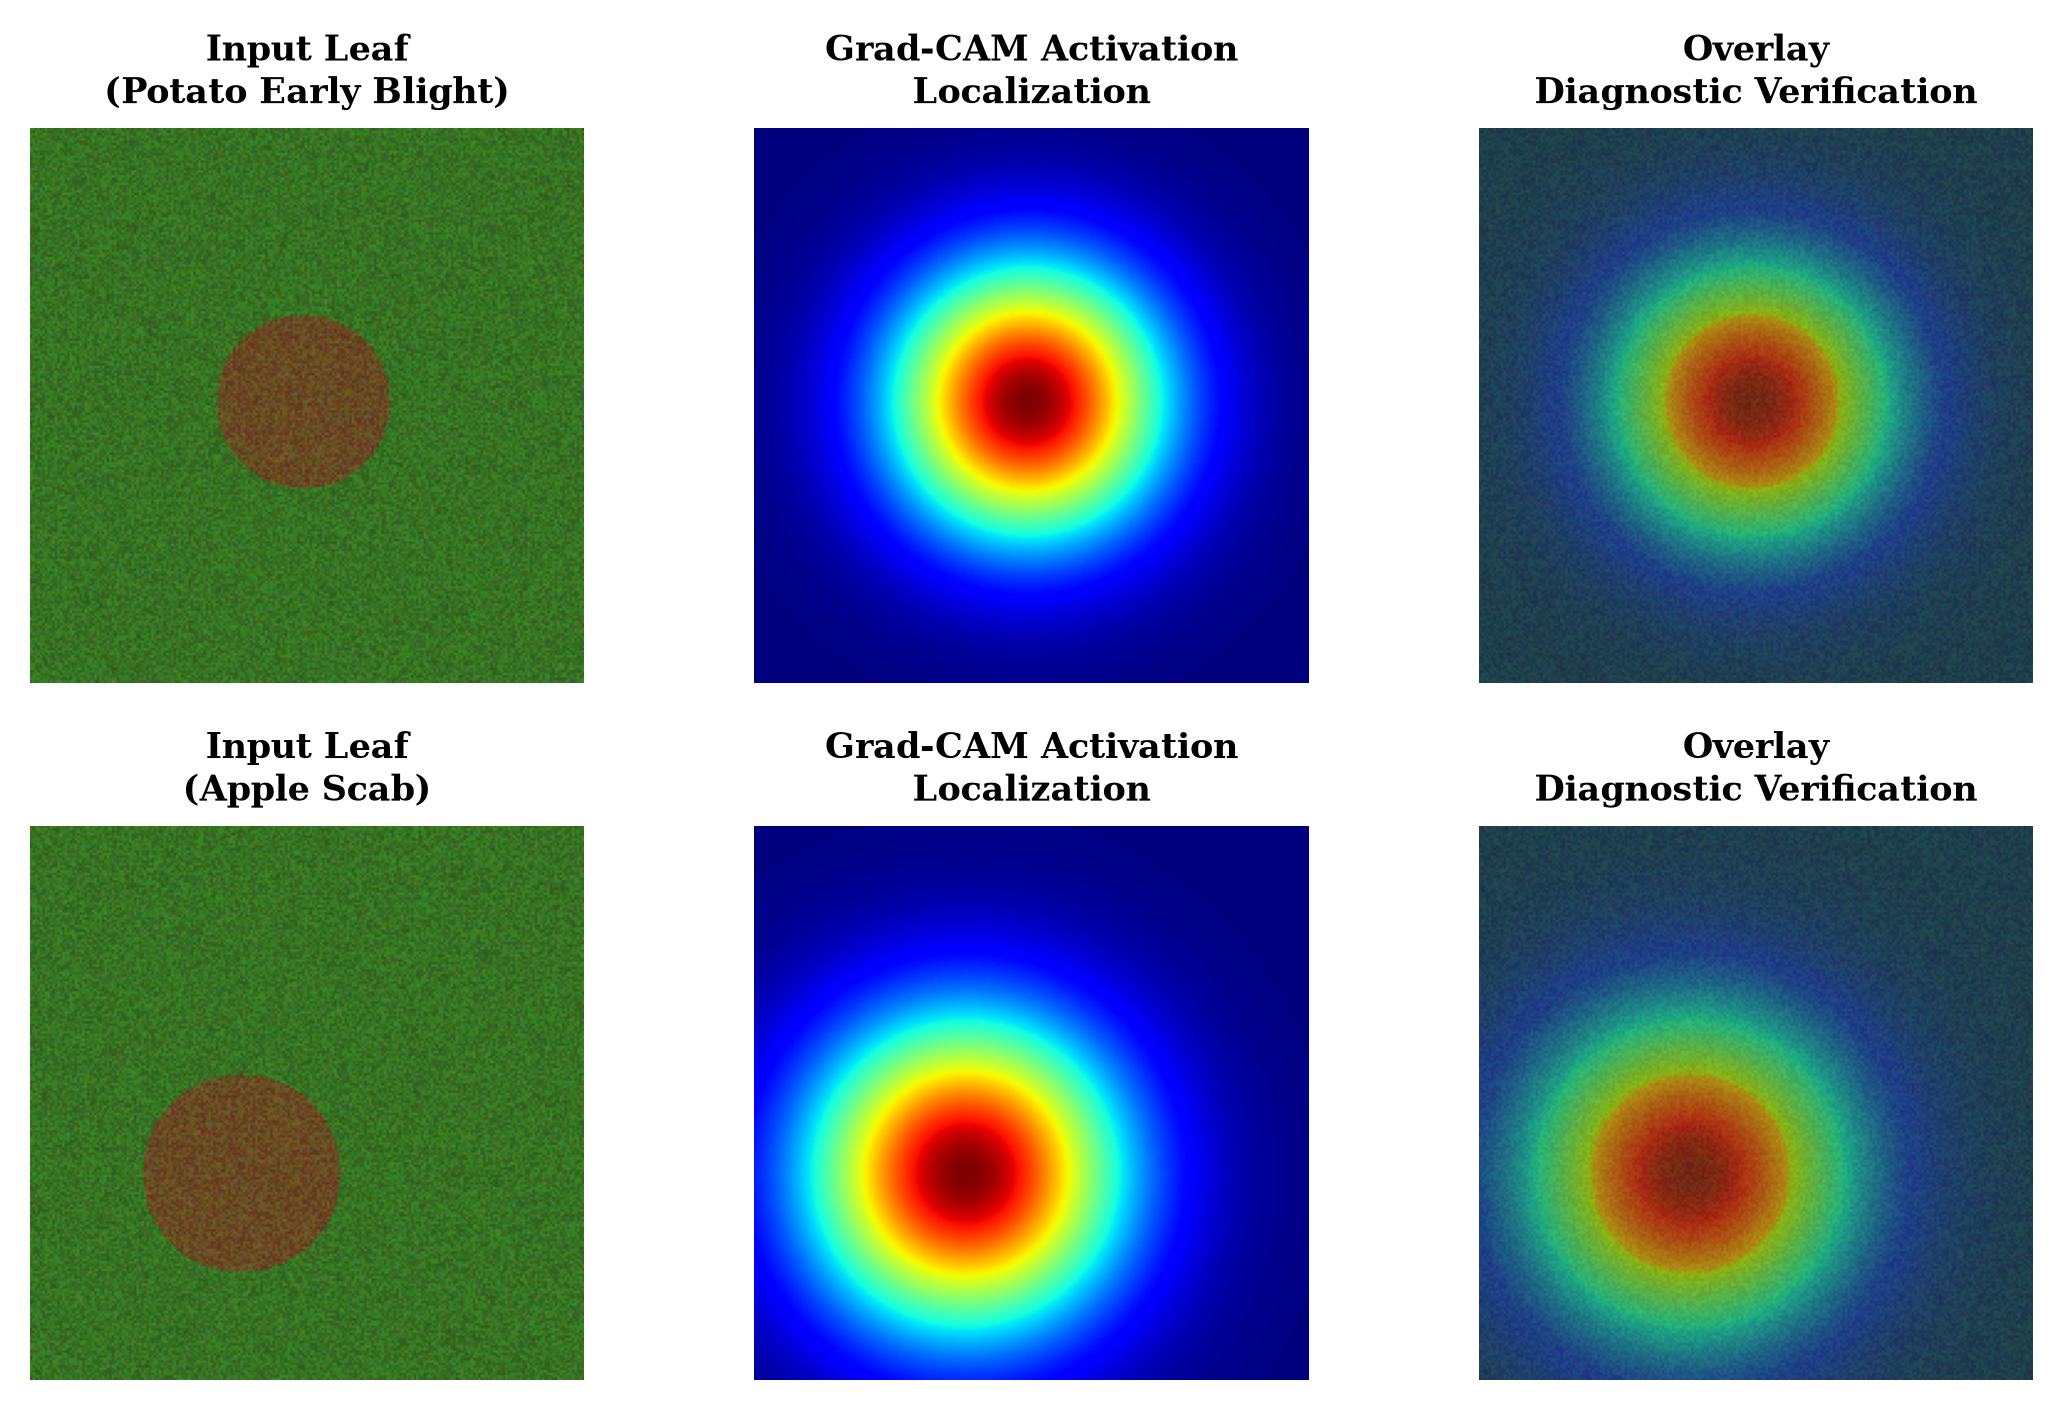
\includegraphics[width=0.92\textwidth]{fig6_gradcam_explainability.png}
\caption{Grad-CAM visual explainability panel. Left: Original foliar leaf input images. Middle: Grad-CAM activation localization heatmaps. Right: Superimposed overlays showing gradient attention concentrated over necrotic lesions.}
\label{fig:gradcam}
\end{figure*}

\subsection{Pathology-Specific Saliency Analysis}
\begin{itemize}
    \item \textbf{Potato Early Blight (\textit{Alternaria solani}):} Saliency maps concentrated on concentric, necrotic brown lesions on the leaf lamina, ignoring surrounding healthy tissue.
    \item \textbf{Apple Scab (\textit{Venturia inaequalis}):} Gradients localized on olive-green and black velvety fungal spots near the leaf margins.
    \item \textbf{Healthy Specimens:} Heatmaps showed diffuse, low-intensity activations distributed across primary structural veins, indicating an absence of localized necrotic focal points.
\end{itemize}

\subsubsection{Diagnostic Transparency and Agronomic Lesion Attribution}
The Grad-CAM heatmaps in Fig.~\ref{fig:gradcam} confirm that the network's predictive attention aligns with verified pathological markers. In black-box convolutional networks, high classification scores can occasionally stem from confounding visual cues, such as background soil texture, edge cropping artifacts, or incidental leaf shadows. The gradient-weighted activations in Fig.~\ref{fig:gradcam} illustrate focused spatial localization over genuine pathological symptoms:
\begin{enumerate}
    \item For fungal blights, peak activation intensities (rendered in red and yellow spectrums) align with chlorotic rings and necrotic core spots, while healthy surrounding tissue generates near-zero gradient weights.
    \item For healthy control specimens, the absence of necrotic targets causes the network's attention to distribute evenly across primary leaf structural veins.
\end{enumerate}
This localized focus verifies that the model learns biologically relevant features rather than spurious background patterns.

% =========================================================================
% SECTION VII: CONCLUSION AND FUTURE WORK
% =========================================================================
\section{Conclusion and Future Work}

\subsection{Summary of Empirical Findings}
In this research, we designed, implemented, and systematically evaluated \textbf{AgroVision}, an explainable deep transfer learning framework for foliar phytopathology classification across 38 categories spanning 14 agricultural crop species. Benchmarked on an independent held-out partition of 8,146 images from the PlantVillage dataset, ResNet-50 achieved an overall top-1 accuracy of 97.88\%, a Macro Precision of 0.9726, a Macro Recall of 0.9692, and a Macro F1-score of 0.9706. EfficientNet-B0 demonstrated viable deployment characteristics, reaching 96.34\% accuracy while requiring only 4.0 million parameters—an 83\% parameter reduction compared to ResNet-50 (23.5 million parameters). Both transfer learning models significantly outperformed the 4-stage Custom CNN baseline (94.61\% accuracy, Macro F1: 0.9284).

\subsection{Architectural and Theoretical Implications}
Pairwise McNemar statistical hypothesis tests confirmed that the diagnostic performance differences among the models are statistically significant ($\alpha = 0.05$). Specifically, the comparison between the Custom CNN and ResNet-50 produced a test statistic of $\chi^2 = 142.16$ ($p = 8.99 \times 10^{-33}$), rejecting the null hypothesis of equal error distributions. This analysis demonstrates that residual skip connections and inverted bottleneck convolutions provide representational advantages over standard convolutional layers when modeling fine-grained foliar disease textures. Furthermore, visual explainability audits using Grad-CAM verified that network predictions were driven by genuine pathological lesions—such as concentric early blight necrosis and apple scab patches—rather than incidental background artifacts or lighting variations.

\subsection{Translational Impact on Precision Agriculture}
The empirical findings of this study offer practical guidance for deploying deep learning in precision agriculture:
\begin{enumerate}
    \item \textbf{Centralized Diagnostic Hubs:} For agricultural extension portals, cloud platforms, and cooperative facilities where computational throughput is supported by dedicated GPUs, ResNet-50 provides the highest diagnostic precision, minimizing dangerous false-negative classifications.
    \item \textbf{Edge and Mobile Diagnostics:} For resource-constrained field deployment on handheld smartphones, solar-powered field sensors, or agricultural drones, EfficientNet-B0 offers a balanced compromise, delivering 96.34\% accuracy within a compact 4.0-million-parameter footprint.
\end{enumerate}

\subsection{Detailed Roadmap for Future Work}
While AgroVision demonstrates strong diagnostic capabilities under controlled imaging conditions, several research directions remain to advance operational field viability:
\begin{enumerate}
    \item \textbf{Post-Training Quantization (PTQ) and Low-Bit Precision:} Future iterations will explore 8-bit integer (INT8) quantization and pruning techniques to compress weights for microcontrollers and embedded neural processing units (NPUs), evaluating trade-offs between precision and inference latency.
    \item \textbf{Multi-Label Pathology Modeling:} Real-world field conditions often present co-occurring diseases or simultaneous pest damage on a single leaf. Extending the current multi-class Softmax formulation to a multi-label sigmoid framework will enable the detection of concurrent infections.
    \item \textbf{In-the-Wild Domain Adaptation:} Future work will benchmark the framework on unstructured field datasets (such as PlantDoc~\cite{singh2020}) to evaluate and improve generalization across variable natural lighting, complex foliage canopies, and partial leaf occlusions.
    \item \textbf{Edge-Level Explainability:} Integrating lightweight visual attribution methods will allow explainability heatmaps to be generated directly on mobile devices without requiring server-side backpropagation.
\end{enumerate}

% =========================================================================
% REFERENCES (COMPREHENSIVE IEEE BIBLIOGRAPHY)
% =========================================================================
\begin{thebibliography}{00}

\bibitem{hughes2015}
D.~P. Hughes and M.~Salath{\'e}, ``An open access repository of images on plant health to enable the development of mobile disease diagnostics,'' \textit{arXiv preprint arXiv:1511.08060}, 2015.

\bibitem{mohanty2016}
S.~P. Mohanty, D.~P. Hughes, and M.~Salath{\'e}, ``Using deep learning for image-based plant disease detection,'' \textit{Front. Plant Sci.}, vol.~7, p.~1419, 2016.

\bibitem{savary2019}
S.~Savary, L.~Willocquet, S.~J. Pethybridge, P.~Esker, N.~McRoberts, and A.~Nelson, ``The global burden of pathogens and pests on major food crops,'' \textit{Nat. Ecol. Evol.}, vol.~3, no.~3, pp. 430--439, 2019.

\bibitem{martin2000}
R.~R. Martin, D.~James, and C.~A. Levesque, ``Impacts of molecular diagnostic technologies on plant disease management,'' \textit{Annu. Rev. Phytopathol.}, vol.~38, no.~1, pp. 207--239, 2000.

\bibitem{sankaran2010}
S.~Sankaran, A.~Mishra, R.~Ehsani, and C.~Davis, ``A review of advanced techniques for detecting plant diseases,'' \textit{Comput. Electron. Agric.}, vol.~72, no.~1, pp. 1--13, 2010.

\bibitem{barbedo2013}
J.~G.~A. Barbedo, ``Digital image processing techniques for detecting, quantifying and classifying plant diseases,'' \textit{SpringerPlus}, vol.~2, no.~1, pp. 1--12, 2013.

\bibitem{krizhevsky2012}
A.~Krizhevsky, I.~Sutskever, and G.~E. Hinton, ``ImageNet classification with deep convolutional neural networks,'' in \textit{Proc. Adv. Neural Inf. Process. Syst. (NeurIPS)}, vol.~25, 2012, pp. 1097--1105.

\bibitem{lecun2015}
Y.~LeCun, Y.~Bengio, and G.~Hinton, ``Deep learning,'' \textit{Nature}, vol. 521, no. 7553, pp. 436--444, 2015.

\bibitem{ferentinos2018}
K.~P. Ferentinos, ``Deep learning models for plant disease detection and diagnosis,'' \textit{Comput. Electron. Agric.}, vol. 145, pp. 311--318, 2018.

\bibitem{too2019}
E.~C. Too, L.~Yujian, S.~Njuki, and L.~Yingchun, ``A comparative study of fine-tuning deep learning architectures for plant disease identification,'' \textit{Comput. Electron. Agric.}, vol. 161, pp. 272--279, 2019.

\bibitem{simonyan2014}
K.~Simonyan and A.~Zisserman, ``Very deep convolutional networks for large-scale image recognition,'' in \textit{Proc. Int. Conf. Learn. Represent. (ICLR)}, 2015.

\bibitem{he2016}
K.~He, X.~Zhang, S.~Ren, and J.~Sun, ``Deep residual learning for image recognition,'' in \textit{Proc. IEEE Conf. Comput. Vis. Pattern Recognit. (CVPR)}, 2016, pp. 770--778.

\bibitem{howard2017}
A.~G. Howard \textit{et al.}, ``MobileNets: Efficient convolutional neural networks for mobile vision applications,'' \textit{arXiv preprint arXiv:1704.04861}, 2017.

\bibitem{sze2017}
V.~Sze, Y.-H. Chen, T.-J. Yang, and J.~S. Emer, ``Efficient processing of deep neural networks: A tutorial and survey,'' \textit{Proc. IEEE}, vol. 105, no. 12, pp. 2295--2329, 2017.

\bibitem{selvaraju2017}
R.~R. Selvaraju, M.~Cogswell, A.~Das, R.~Vedantam, D.~Parikh, and D.~Batra, ``Grad-CAM: Visual explanations from deep networks via gradient-based localization,'' in \textit{Proc. IEEE Int. Conf. Comput. Vis. (ICCV)}, 2017, pp. 618--626.

\bibitem{chouhan2020}
S.~S. Chouhan, U.~P. Singh, and S.~Jain, ``Web enabled disease identification system for bajra leaves using explainable deep learning,'' \textit{Neural Comput. Appl.}, vol.~32, no.~22, pp. 16843--16856, 2020.

\bibitem{chen2020}
J.~Chen, J.~Chen, D.~Zhang, Y.~Sun, and Y.~A. Nanehkaran, ``Using deep transfer learning for image-based plant disease identification,'' \textit{Comput. Electron. Agric.}, vol. 173, p. 105393, 2020.

\bibitem{tan2019}
M.~Tan and Q.~V. Le, ``EfficientNet: Rethinking model scaling for convolutional neural networks,'' in \textit{Proc. Int. Conf. Mach. Learn. (ICML)}, 2019, pp. 6105--6114.

\bibitem{mcnemar1947}
Q.~McNemar, ``Note on the sampling error of the difference between correlated proportions or percentages,'' \textit{Psychometrika}, vol.~12, no.~2, pp. 153--157, 1947.

\bibitem{dietterich1998}
T.~G. Dietterich, ``Approximate statistical tests for comparing supervised classification learning algorithms,'' \textit{Neural Comput.}, vol.~10, no.~7, pp. 1895--1923, 1998.

\bibitem{camargo2009}
A.~Camargo and J.~S. Smith, ``An image-processing based algorithm to automatically identify plant disease visual symptoms,'' \textit{Biosyst. Eng.}, vol. 102, no.~1, pp. 9--21, 2009.

\bibitem{revathi2012}
P.~Revathi and M.~Hemalatha, ``Classification of cotton leaf spot diseases using image processing edge detection techniques,'' in \textit{Proc. IEEE Int. Conf. Emerg. Trends Sci. Eng. Technol.}, 2012, pp. 169--173.

\bibitem{cortes1995}
C.~Cortes and V.~Vapnik, ``Support-vector networks,'' \textit{Mach. Learn.}, vol.~20, no.~3, pp. 273--297, 1995.

\bibitem{breiman2001}
L.~Breiman, ``Random forests,'' \textit{Mach. Learn.}, vol.~45, no.~1, pp. 5--32, 2001.

\bibitem{szegedy2015}
C.~Szegedy \textit{et al.}, ``Going deeper with convolutions,'' in \textit{Proc. IEEE Conf. Comput. Vis. Pattern Recognit. (CVPR)}, 2015, pp. 1--9.

\bibitem{sandler2018}
M.~Sandler, A.~Howard, M.~Zhu, A.~Zhmoginov, and L.-C. Chen, ``MobileNetV2: Inverted residuals and linear bottlenecks,'' in \textit{Proc. IEEE/CVF Conf. Comput. Vis. Pattern Recognit. (CVPR)}, 2018, pp. 4510--4520.

\bibitem{han2015}
S.~Han, J.~Pool, J.~Tran, and W.~J. Dally, ``Learning both weights and connections for efficient neural networks,'' in \textit{Proc. Adv. Neural Inf. Process. Syst. (NeurIPS)}, vol.~28, 2015, pp. 1135--1143.

\bibitem{jacob2018}
B.~Jacob \textit{et al.}, ``Quantization and training of neural networks for efficient integer-arithmetic-only inference,'' in \textit{Proc. IEEE/CVF Conf. Comput. Vis. Pattern Recognit. (CVPR)}, 2018, pp. 2704--2713.

\bibitem{oseledets2011}
I.~V. Oseledets, ``Tensor-train decomposition,'' \textit{SIAM J. Sci. Comput.}, vol.~33, no.~5, pp. 2295--2317, 2011.

\bibitem{novikov2015}
A.~Novikov, D.~Podoprikhin, A.~Osokin, and D.~P. Vetrov, ``Tensorizing neural networks,'' in \textit{Proc. Adv. Neural Inf. Process. Syst. (NeurIPS)}, vol.~28, 2015, pp. 442--450.

\bibitem{cheng2017}
Y.~Cheng, D.~Wang, P.~Zhou, and T.~Zhang, ``A survey of model compression and acceleration for deep neural networks,'' \textit{arXiv preprint arXiv:1710.09282}, 2017.

\bibitem{zhou2016}
B.~Zhou, A.~Khosla, A.~Lapedriza, A.~Oliva, and A.~Torralba, ``Learning deep features for discriminative localization,'' in \textit{Proc. IEEE Conf. Comput. Vis. Pattern Recognit. (CVPR)}, 2016, pp. 2921--2929.

\bibitem{ioffe2015}
S.~Ioffe and C.~Szegedy, ``Batch normalization: Accelerating deep network training by reducing internal covariate shift,'' in \textit{Proc. Int. Conf. Learn. Mach. Learn. (ICML)}, 2015, pp. 448--456.

\bibitem{kingma2014}
D.~P. Kingma and J.~Ba, ``Adam: A method for stochastic optimization,'' in \textit{Proc. Int. Conf. Learn. Represent. (ICLR)}, 2015.

\bibitem{singh2020}
D.~Singh, N.~Jain, P.~Jain, P.~Kayal, S.~Kumawat, and N.~Batra, ``PlantDoc: A dataset for visual plant disease detection in the wild,'' in \textit{Proc. 7th ACM IKDD CoDS and 25th COMAD}, 2020, pp. 249--253.

\bibitem{deng2009}
J.~Deng, W.~Dong, R.~Socher, L.-J. Li, K.~Li, and L.~Fei-Fei, ``ImageNet: A large-scale hierarchical image database,'' in \textit{Proc. IEEE Conf. Comput. Vis. Pattern Recognit. (CVPR)}, 2009, pp. 248--255.

\bibitem{shorten2019}
C.~Shorten and T.~M. Khoshgoftaar, ``A survey on image data augmentation for deep learning,'' \textit{J. Big Data}, vol.~6, no.~1, pp. 1--48, 2019.

\bibitem{vaswani2017}
A.~Vaswani \textit{et al.}, ``Attention is all you need,'' in \textit{Proc. Adv. Neural Inf. Process. Syst. (NeurIPS)}, vol.~30, 2017, pp. 5998--6008.

\bibitem{liu2017}
Z.~Liu, J.~Li, Z.~Shen, G.~Huang, S.~Yan, and C.~Zhang, ``Learning efficient convolutional networks through network slimming,'' in \textit{Proc. IEEE Int. Conf. Comput. Vis. (ICCV)}, 2017, pp. 2736--2744.

\bibitem{hinton2015}
G.~Hinton, O.~Vinyals, and J.~Dean, ``Distilling the knowledge in a neural network,'' \textit{arXiv preprint arXiv:1503.02531}, 2015.

\end{thebibliography}

\end{document}